\section{Parte I}
    \subsection{Gráfico}
        \begin{figure} [H] 
            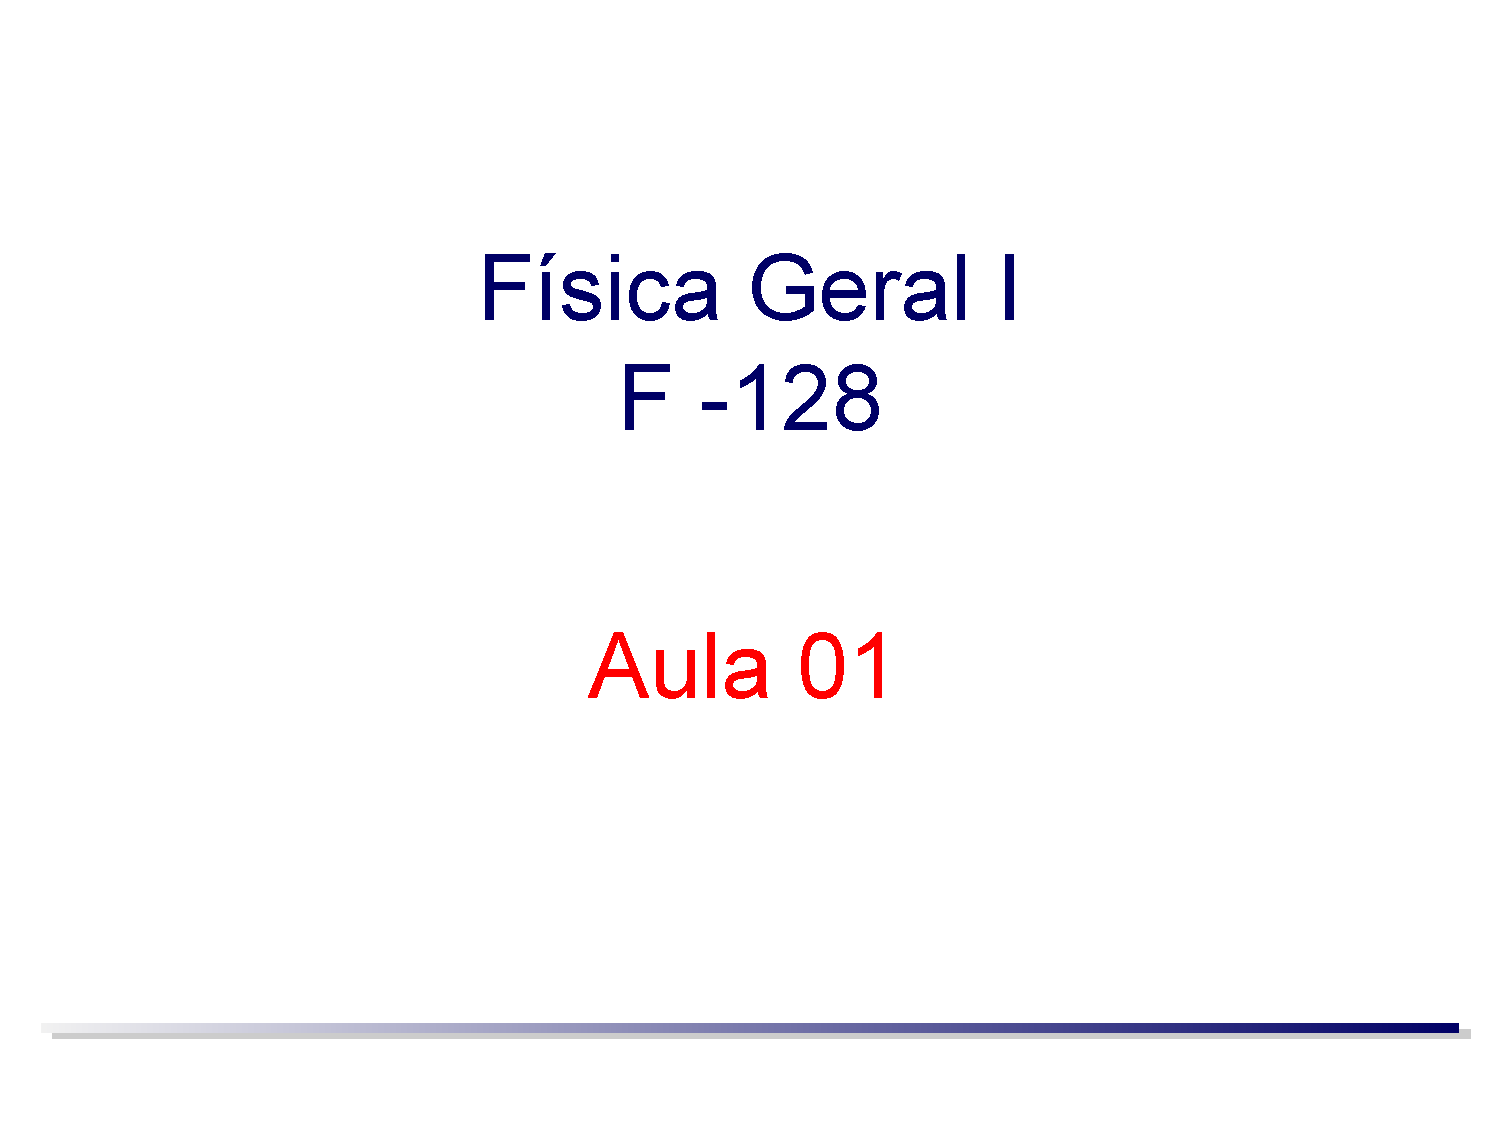
\includegraphics[width=\textwidth]{01}
            \caption{Gráfico de $t$ por $ln(V_{cap})$}
            \label{fig:01}
        \end{figure}
    \subsection{A constante de tempo}
       
        Ao observar os coeficientes do gráfico pode-se determinar a 
        constante de tempo como sendo $-\frac{1}{A}$. 
        Pois pela linearização da equação:

        $$V_c = \epsilon \times exp(-\frac{1}{RC})$$

        Obtemos:

        $$ln(V_c) = ln(\epsilon) - \frac{t}{RC}$$

        Dessa forma, obtem-se o valor de RC como $\frac{-1}{-1}$, sendo assim:
        
        $$\tau = 1,00s$$

        Para obter o seu erro deriva-se parcialmente a equação $\tau = -\frac{1}{A}$
        em função de A, assim: 

        $$\Delta\tau^2 = (\frac{1}{A^4})\times\Delta A^2 
        \Rightarrow \Delta\tau = \frac{\Delta A}{A^2}$$

        Portanto, seu erro é: 
        
        $$\Delta\tau = 0,01s$$
        
        Conclui-se que experimentalmente RC equivale a 
        
        $$RC = \tau = (1,00 \pm 0,01)s$$

    \subsection{Constante de tempo vs valor esperado}
        
        O valor teórico da constante de tempo é obtido através da 
        Resistência e Capacitancia verificadas pelo multimetro.
        Dessa forma seus valores nominais são $R = (998 \pm 3)\Omega$ 
        e $C = (0,966 \pm 0,003)mF$, os erros foram obtidos através 
        do manual e a probabilidade retangular. Assim:
        
        $$\tau = RC = 0,964s$$

        E seu erro:

        $$\Delta\tau = (\frac{\partial\tau}{\partial R})^2 \times \Delta R^2
        + (\frac{\partial\tau}{\partial C})^2\times\Delta C^2$$

        Logo:

        $$\Delta\tau = 0,04s$$

        Portanto:

        $$\tau = (0,96 \pm 0,04)s$$

        O valor teórico comparado com o experimental acabam por coincidir 
        dentro dos erros esperados.
        
            $$\tau_{experimental} = (1,00 \pm 0,01)s$$
            $$\tau_{teorico} = (0,96 \pm 0,04)s$$